% ============================================================================
% Solving Nonlinear DSGE Models with DEQNs: The IRBC Model
% Duration: 60 minutes
% ============================================================================

\documentclass[aspectratio=169,11pt]{beamer}

% ---------- Theme and colors ----------
\usecolortheme{dove}
\setbeamertemplate{navigation symbols}{}
\setbeamertemplate{footline}{%
  \hfill\usebeamerfont{page number in head/foot}%
  \usebeamercolor[fg]{normal text}%
  \insertframenumber\,/\,\inserttotalframenumber\kern1em\vskip4pt}
\setbeamerfont{frametitle}{size=\huge}

% ---------- Packages ----------
\usepackage[utf8]{inputenc}
\usepackage[T1]{fontenc}
\usepackage{amsmath,amssymb,amsfonts}
\usepackage{bm}
\usepackage{graphicx}
\usepackage{tikz}
\usetikzlibrary{shapes,arrows.meta,positioning,calc,fit,backgrounds,patterns,decorations.pathreplacing}
\usepackage{pgfplots}
\pgfplotsset{compat=1.18}
\usepackage{booktabs}
\usepackage{hyperref}
\usepackage{multicol}
\usepackage{xcolor}
\usepackage{algorithm}
\usepackage{algorithmic}
\usepackage{listings}

% ---------- Listings style for Python ----------
\lstset{
    language=Python,
    basicstyle=\small\ttfamily,
    keywordstyle=\color{uzhblue}\bfseries,
    commentstyle=\color{uzhgreydark}\itshape,
    stringstyle=\color{darkgreen},
    showstringspaces=false,
    breaklines=true,
    frame=none,
    xleftmargin=0pt,
    aboveskip=4pt,
    belowskip=4pt,
    escapeinside={(*@}{@*)},
}

% ---------- Custom colors ----------
\definecolor{uzhblue}{rgb}{0,0,0.5}
\definecolor{uzhgreylight}{RGB}{236,238,241}
\definecolor{uzhgreydark}{RGB}{81,86,94}
\definecolor{harvardcrimson}{RGB}{153,0,0}
\definecolor{unil@blue}{RGB}{0,140,204}
\definecolor{unil@black}{RGB}{35,31,32}
\definecolor{darkgreen}{RGB}{0,100,0}
\definecolor{darkred}{RGB}{139,0,0}
\definecolor{softblue}{RGB}{70,130,180}
\definecolor{softorange}{RGB}{230,159,0}
\definecolor{softgreen}{RGB}{0,158,115}

% ---------- Set beamer colors ----------
\setbeamercolor{frametitle}{bg=uzhgreylight, fg=uzhblue}
\setbeamercolor{title}{fg=uzhblue}
\setbeamercolor{structure}{fg=uzhblue}
\setbeamercolor{block title}{bg=unil@blue, fg=white}
\setbeamercolor{block body}{bg=uzhgreylight}
\setbeamercolor{block title alerted}{bg=darkred,fg=white}
\setbeamercolor{block body alerted}{bg=red!5}
\setbeamercolor{block title example}{bg=darkgreen,fg=white}
\setbeamercolor{block body example}{bg=green!5}
\setbeamercolor{item}{fg=unil@black}
\setbeamercolor{normal text}{fg=unil@black}

% ---------- Emphasis and hyperlinks ----------
\newcommand{\emphc}[1]{\textcolor{harvardcrimson}{#1}}
\hypersetup{colorlinks,linkcolor=harvardcrimson,urlcolor=harvardcrimson}

% ---------- Math commands ----------
\newcommand{\x}{\bm{x}}
\newcommand{\w}{\bm{w}}
\newcommand{\bb}{\bm{b}}
\newcommand{\z}{\bm{z}}
\newcommand{\W}{\bm{W}}
\newcommand{\X}{\bm{X}}
\renewcommand{\a}{\bm{a}}
\newcommand{\R}{\mathbb{R}}
\newcommand{\E}[1]{\mathbb{E}\!\left[#1\right]}
\DeclareMathOperator*{\argmin}{arg\,min}
\DeclareMathOperator*{\argmax}{arg\,max}

% ---------- Title ----------
\title[IRBC -- Padova 2026]%
{Deep Learning for Solving Dynamic Models}
\subtitle{Session 5: Scaling up, the international real business cycle model}
\author{Simon Scheidegger}
\institute[HEC Lausanne]{HEC, University of Lausanne}
\date{University of Padova\\September 23, 2026}

\begin{document}
% --- Exercise pause badge ---
\newcommand{\exercisepause}{%
  \tikz[baseline=(X.base)]{\node[fill=darkgreen!80!black, text=white,
  rounded corners=2pt, inner sep=3pt, font=\scriptsize\bfseries](X){PAUSE, 5 min};}}


% ============================================================================
% PART 0: TITLE & OUTLINE
% ============================================================================

% --- Slide 1: Title ---
{\setbeamercolor{background canvas}{bg=uzhgreylight}
\begin{frame}
\titlepage
\vspace{-0.4cm}
\begin{center}
{\footnotesize Based on: Azinovic, Gaegauf \& Scheidegger (2022), \emph{International Economic Review} 63(4), 1471--1525.\\
Brumm, Krause, Schaab \& Scheidegger (2022), ``Sparse Grids for Dynamic Economic Models,'' \emph{Oxford Research Encyclopedia of Economics and Finance}, Oxford University Press.}
\end{center}
\end{frame}
}

% --- Slide 2: Roadmap ---
\begin{frame}{Roadmap of This Lecture}
\vspace{0.2em}
\begin{columns}[T]
\column{0.48\textwidth}
\textbf{Part A}
\begin{itemize}
    \item \textbf{Part I.} The IRBC model: preferences, production, TFP, adjustment costs, irreversibility, Fischer--Burmeister
    \item Equilibrium system + finger exercise
\end{itemize}

\column{0.48\textwidth}
\textbf{Part B}
\begin{itemize}
    \item \textbf{Part II.} DEQN formulation: states, architecture, loss, Gauss--Hermite, training algorithm
    \item \textbf{Part III.} Implementation: Keras code, convergence, policy functions, validation
    \item Bridge to the production-code DEQN library
\end{itemize}
\end{columns}
\end{frame}

% --- Learning objectives ---
\begin{frame}{Learning objectives}
\textbf{By the end of this lecture you should be able to:}
\begin{itemize}
  \item Set up the International Real Business Cycle model with multi-country state space, capital adjustment costs, and irreversibility constraints
  \item Derive first-order conditions (Euler equations, consumption sharing) and convert KKT conditions into smooth complementarity functions (Fischer--Burmeister)
  \item Formulate the DEQN loss function for multi-country DSGE models and train the network on simulated paths
  \item Implement policy functions in Keras and validate numerical solutions against theoretical steady states
  \item Extend the framework to 4--100+ dimensional problems and perform sensitivity analysis on model parameters
\end{itemize}
\end{frame}


% ============================================================================
% PART I: THE IRBC MODEL
% ============================================================================

% --- Slide 4: Section Divider ---
\begin{frame}{}
\vfill
\begin{center}
{\Huge \textcolor{uzhblue}{\textbf{Part I}}}\\[12pt]
{\LARGE The IRBC Model}
\end{center}
\vfill
\end{frame}

% --- Slide 5: Why International Models? ---
\begin{frame}{Why International Models, and Why IRBC as a Testbed?}
\scriptsize
\begin{columns}[T]
\column{0.50\textwidth}
\textbf{The economics.}  Capital flows, international risk sharing and trade imbalances all need
$N$ heterogeneous countries linked through a world capital market. The IRBC model is the workhorse:
\begin{itemize}\itemsep1pt
    \item \emphc{Consumption-correlation puzzle} (Backus--Kehoe--Kydland 1992): complete markets
          imply $\rho(c^i,c^j)\approx 1$; data say $\rho(c^i,c^j)<\rho(y^i,y^j)$.
    \item \emphc{Home bias} and the \emphc{welfare cost of missing insurance} (Heathcote \& Perri 2002).
    \item Macro-financial transmission through adjustment costs, constraints, Pareto weights.
\end{itemize}

\vspace{0.2em}
\textbf{The computation.}  State dimension is \emphc{linear in $N$}: $2N$, capital and TFP per country.
Smooth but highly nonlinear; the planner's problem gives a clean target; the standard benchmark for
projection methods (Krueger \& K\"ubler 2004; Brumm \& Scheidegger 2017).

\column{0.46\textwidth}
\begin{center}
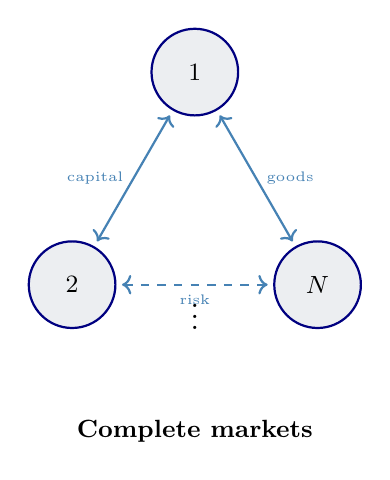
\begin{tikzpicture}[
    country/.style={circle, draw=uzhblue, thick, fill=uzhgreylight,
        minimum size=1.1cm, font=\small},
    flow/.style={<->, thick, softblue, shorten >=2pt, shorten <=2pt}
]
    \node[country] (c1) at (90:1.8) {$1$};
    \node[country] (c2) at (210:1.8) {$2$};
    \node[country] (c3) at (330:1.8) {$N$};
    \node[font=\large] at (270:1.2) {$\vdots$};
    \draw[flow] (c1) -- (c2) node[midway, left, font=\tiny] {capital};
    \draw[flow] (c1) -- (c3) node[midway, right, font=\tiny] {goods};
    \draw[flow, dashed] (c2) -- (c3) node[midway, below, font=\tiny] {risk};
    \node[below=0.3cm, font=\small\bfseries] at (0,-2.2) {Complete markets};
\end{tikzpicture}
\end{center}
\end{columns}
\end{frame}

% --- Slide 5b: IRBC in Macro-Finance ---
% --- Padova cut: frame "Why IRBC for Macro-Finance Research?" (13 lines) commented out ---
% \begin{frame}{Why IRBC for Macro-Finance Research?}
% \footnotesize
% Workhorse for \emphc{open-economy asset pricing} and \emphc{international risk sharing}:
% 
% \vspace{0.2em}
% \begin{itemize}\itemsep0pt
%     \item \textbf{International risk sharing.}  Complete markets imply perfectly correlated consumption; data do not (Backus, Kehoe \& Kydland 1992).
%     \item \textbf{Market structure \& welfare.}  Complete vs.\ incomplete markets; welfare cost of missing insurance (Heathcote \& Perri 2002).
%     \item \textbf{Capital flows \& current account} from intertemporal savings + heterogeneous productivity.
%     \item \textbf{Home bias}: frictionless benchmark for observed portfolio holdings.
%     \item \textbf{Macro-financial transmission} via adjustment costs, constraints, Pareto weights.
% \end{itemize}
% \end{frame}

% --- Slide 5c: IRBC as a computational testbed ---
% --- Padova cut: frame "IRBC: Puzzles and Computational Testbed" (22 lines) commented out ---
% \begin{frame}{IRBC: Puzzles and Computational Testbed}
% \footnotesize
% \begin{columns}[T]
% \column{0.49\textwidth}
% \textbf{Macro-finance puzzles:}
% \begin{itemize}\itemsep2pt
%     \item \emphc{Consumption-correlation puzzle} (Backus--Kehoe--Kydland 1992):
%     complete markets imply $\rho(c^i,c^j)\!\approx\!1$, but in the data $\rho(c^i,c^j)<\rho(y^i,y^j)$.
%     \item \emphc{Portfolio home-bias puzzle}: optimal diversification predicts large foreign-equity holdings; observed portfolios are strongly domestic.
%     \item \emphc{Real-exchange-rate (RER) volatility} (Backus--Smith): the ratio of price levels $P^j/P^i$ is far more volatile than the consumption ratio $c^j/c^i$; IRBC with nontraded goods (Stockman \& Tesar, 1995) reproduces this.
% \end{itemize}
% 
% \column{0.49\textwidth}
% \textbf{Computational testbed:}
% \begin{itemize}\itemsep0pt
%     \item State dim.\ \emphc{linear} in $N$: $2N$.
%     \item Smooth but \emphc{highly nonlinear}.
%     \item \emphc{Planner} gives a clean target.
%     \item Benchmark for projection methods (Krueger \& Kubler 2004; Brumm \& Scheidegger 2017).
% \end{itemize}
% \end{columns}
% \end{frame}

% --- Slide 6: Model Overview ---
\begin{frame}{Model Overview}
\textbf{International Real Business Cycle (IRBC) model}: Backus, Kehoe \& Kydland (1992); here with the DEQN-style extensions of Azinovic, Gaegauf \& Scheidegger (2022):

\vspace{0.5em}
\begin{itemize}
    \item $N$ countries, each with \emphc{country-specific capital} $k^j$ and \emphc{TFP} $z^j$
    \item \emphc{Complete markets}: a social planner allocates resources with Pareto weights $\tau^j$
    \item \emphc{Irreversible investment}: $I^j \geq 0$ (cannot disinvest)
    \item \emphc{Capital adjustment costs}: $\Gamma^j = \frac{\kappa}{2} k^j \!\left(\frac{k^{j\prime}}{k^j} - 1\right)^{\!2}$
\end{itemize}

\vspace{0.5em}
\begin{block}{Dimensionality}
State: $\bm{s} = (k^1, \ldots, k^N, z^1, \ldots, z^N) \in \R^{2N}$\\
Policy: $(k^{1\prime}, \ldots, k^{N\prime}, \lambda, \mu^1, \ldots, \mu^N) \in \R^{2N+1}$
\end{block}
\end{frame}

% --- Slide 7: Preferences ---
\begin{frame}{Preferences}
\small
Each country $j$ has \emphc{CRRA utility} (with the standard log limit at $\gamma_j = 1$):
\[
u^j(c) \;=\; \begin{cases} \dfrac{c^{\,1 - 1/\gamma_j} - 1}{1 - 1/\gamma_j}, & \gamma_j \neq 1, \\[4pt] \ln c, & \gamma_j = 1. \end{cases}
\]

\vspace{0.2em}
\begin{itemize}\itemsep2pt
    \item $\gamma_j$: intertemporal elasticity of substitution for country $j$
    \item \emphc{Heterogeneous} across countries: $\gamma_j$ linearly spaced in $[0.25, 1.0]$ (so risk aversion $1/\gamma_j \in [1, 4]$; the $\ln c$ branch is used at $\gamma_j = 1$)
\end{itemize}

\vspace{0.2em}
{\scriptsize \emphc{Notation:} in this chapter $\gamma$ is the \textbf{IES}; later chapters on continuous-time HA and climate re-purpose $\gamma$ for CRRA risk aversion (with $\psi$ then the IES). Restated at the top of each chapter.}

\vspace{0.3em}
\textbf{Social planner} maximizes with Pareto weights $\tau^j$:
\[
\max \; \mathbb{E}_0\!\left[\sum_{t=0}^{\infty} \beta^t \sum_{j=1}^{N} \tau^j \, u^j(c_t^j)\right]
\]
\end{frame}

% --- Slide 8: Production ---
\begin{frame}{Production}
Each country $j$ produces a single good:
\[
Y^j = A_{\text{tfp}} \cdot \exp(z^j) \cdot (k^j)^\zeta
\]

\vspace{0.3em}
\textbf{Calibration of $A_{\text{tfp}}$:} chosen so that the \emphc{steady state} is consistent with $k_{ss} = 1$:
\[
\boxed{A_{\text{tfp}} = \frac{1 - \beta(1-\delta)}{\zeta \cdot \beta}}
\]

\vspace{0.5em}
\begin{center}
\begin{tabular}{ll}
\toprule
\textbf{Parameter} & \textbf{Value} \\
\midrule
$\zeta$ (capital share) & 0.36 \\
$\beta$ (discount factor) & 0.99 \\
$\delta$ (depreciation) & 0.01 \\
\bottomrule
\end{tabular}
\end{center}
\end{frame}

% --- Slide 9: TFP Process ---
\begin{frame}{TFP Process}
\begin{columns}[T]
\column{0.48\textwidth}
Log TFP follows an \emphc{AR(1)} with common and idiosyncratic shocks:
\[
z^{j\prime} = \rho_z \, z^j + \sigma_e \bigl(\varepsilon^j + \varepsilon^{\text{agg}}\bigr)
\]

\vspace{0.2em}
\begin{itemize}\itemsep1pt
    \item $\varepsilon^j \sim \mathcal{N}(0,1)$: country-specific
    \item $\varepsilon^{\text{agg}} \sim \mathcal{N}(0,1)$: aggregate shock
    \item Total: $N+1$ independent shocks
\end{itemize}

\vspace{0.2em}
{\small $\rho_z = 0.95$, $\sigma_e = 0.01$}

\vspace{0.2em}
{\scriptsize $\sigma_e$ is the \emph{per-component} std., so the per-country innovation std.\ is $\sigma_e\sqrt{2}$ and the cross-country innovation correlation is $1/2$.}

\column{0.48\textwidth}
\begin{center}
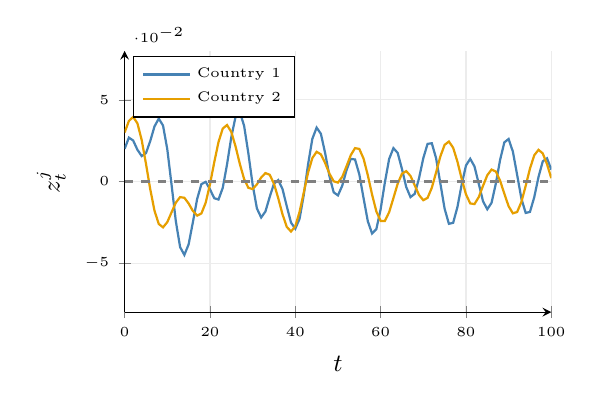
\begin{tikzpicture}
\begin{axis}[
    width=7cm, height=4.9cm,
    xlabel={$t$}, ylabel={$z^j_t$},
    xlabel style={font=\small},
    ylabel style={font=\small},
    tick label style={font=\tiny},
    xmin=0, xmax=100, ymin=-0.08, ymax=0.08,
    grid=major, grid style={gray!15},
    legend style={font=\tiny, at={(0.02,0.98)}, anchor=north west},
    axis lines=left,
]
    \addplot[thick, softblue, domain=0:100, samples=101]
        {0.04*sin(deg(x*0.3))*exp(-0.02*x) + 0.02*cos(deg(x*0.7))};
    \addlegendentry{Country 1}
    \addplot[thick, softorange, domain=0:100, samples=101]
        {0.03*cos(deg(x*0.25))*exp(-0.015*x) + 0.015*sin(deg(x*0.6))};
    \addlegendentry{Country 2}
    \addplot[thick, dashed, gray, domain=0:100]{0};
\end{axis}
\end{tikzpicture}\\
{\tiny Stylized TFP sample paths}
\end{center}
\end{columns}
\end{frame}

% --- Slide 10: Adjustment Costs ---
\begin{frame}{Capital Adjustment Costs}
\begin{columns}[T]
\column{0.48\textwidth}
Changing the capital stock is \emphc{costly} ($\kappa = 0.5$):
\[
\Gamma^j = \frac{\kappa}{2}\, k^j \!\left(\frac{k^{j\prime}}{k^j} - 1\right)^{\!2}
\]

\textbf{Key derivatives:}
\begin{align*}
\frac{\partial \Gamma}{\partial k'} &= \kappa \left(\frac{k'}{k} - 1\right) \\[2pt]
\frac{\partial \Gamma}{\partial k} &= -\frac{\kappa}{2}\left(\frac{k'}{k} - 1\right)\!\left(\frac{k'}{k} + 1\right)
\end{align*}

{\scriptsize\textbf{Role:} smooth investment, break Tobin's $q\!=\!1$, and dampen cross-country \emphc{capital flows}.}

\column{0.48\textwidth}
\begin{center}
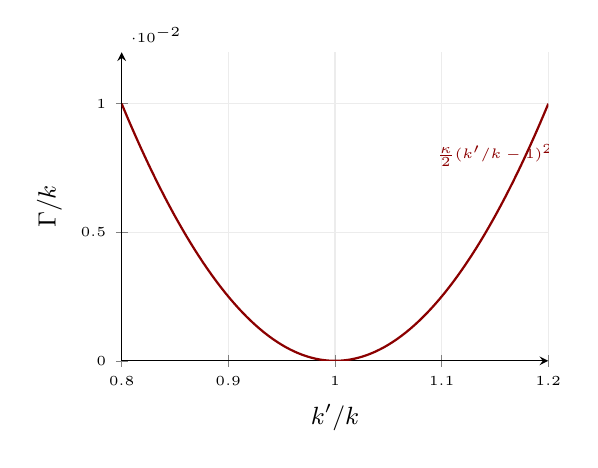
\begin{tikzpicture}
\begin{axis}[
    width=7cm, height=5.5cm,
    xlabel={$k'/k$}, ylabel={$\Gamma / k$},
    xlabel style={font=\small},
    ylabel style={font=\small},
    tick label style={font=\tiny},
    xmin=0.8, xmax=1.2, ymin=0, ymax=0.012,
    grid=major, grid style={gray!15},
    axis lines=left,
]
    \addplot[thick, darkred, domain=0.8:1.2, samples=100]
        {0.25*(x-1)^2};
    \node[font=\tiny, darkred] at (axis cs:1.15,0.008) {$\frac{\kappa}{2}(k'/k-1)^2$};
\end{axis}
\end{tikzpicture}\\
{\tiny Adjustment cost per unit of capital}
\end{center}
\end{columns}
\end{frame}

% --- Slide 11: Putting It Together ---
\begin{frame}{Putting It Together: The Complete Model}
\footnotesize
\textbf{Primitives} (from the previous slides):
\begin{align*}
\text{Preferences:}   &\quad U^j(c) = \tfrac{c^{\,1 - 1/\gamma_j} - 1}{1 - 1/\gamma_j} \\[1pt]
\text{Production:}    &\quad Y_t^j = A_{\mathrm{tfp}}\,\exp(z_t^j)\,(k_t^j)^{\zeta} \\[1pt]
\text{TFP process:}   &\quad z_{t+1}^j = \rho_z\, z_t^j + \sigma_e\bigl(\varepsilon_{t+1}^j + \varepsilon_{t+1}^{\mathrm{agg}}\bigr) \\[1pt]
\text{Adjustment cost:}&\quad \Gamma_t^j = \tfrac{\kappa}{2}\, k_t^j \bigl(k_{t+1}^j/k_t^j - 1\bigr)^{2}
\end{align*}

\textbf{Constraints:}
\begin{align*}
\text{Aggregate resource (ARC):} &\quad \sum_{j=1}^{N}\!\Bigl[ Y_t^j + (1-\delta)\, k_t^j - k_{t+1}^j - \Gamma_t^j - c_t^j \Bigr] = 0 \\[2pt]
\text{Irreversibility:} &\quad I_t^j \equiv k_{t+1}^j - (1-\delta)\, k_t^j \;\geq\; 0 \qquad \forall\, j = 1,\ldots,N
\end{align*}

\smallskip
The planner chooses $\{c_t^j, k_{t+1}^j\}_{j,t}$ subject to these constraints.
\end{frame}

% --- Slide 12: Planner's Problem (dynamic optimization) ---
\begin{frame}{Planner's Problem (Dynamic Optimization)}
\footnotesize
\[
\max_{\{c_t^j,\, k_{t+1}^j\}} \;\; \mathbb{E}_0\!\left[\sum_{t=0}^{\infty} \beta^{t} \sum_{j=1}^{N} \tau^j \, \frac{(c_t^j)^{1 - 1/\gamma_j} - 1}{1 - 1/\gamma_j}\right]
\]
\textbf{subject to:}
\begin{align*}
\text{ARC:} &\quad \sum_{j=1}^{N} \Bigl[ Y_t^j + (1-\delta)\,k_t^j - k_{t+1}^j - \Gamma_t^j - c_t^j \Bigr] = 0 \\[2pt]
\text{Irreversibility:} &\quad k_{t+1}^j - (1-\delta)\,k_t^j \;\geq\; 0 \qquad \forall\, j \\[2pt]
\text{Production:} &\quad Y_t^j = A_{\mathrm{tfp}}\exp(z_t^j)\,(k_t^j)^{\zeta} \\[2pt]
\text{TFP:}         &\quad z_{t+1}^j = \rho_z\, z_t^j + \sigma_e\bigl(\varepsilon_{t+1}^j + \varepsilon_{t+1}^{\mathrm{agg}}\bigr)
\end{align*}

\smallskip
Pareto weights $\tau^j$ allocate welfare across countries. We now \emph{attach multipliers} to the constraints to obtain the first-order conditions.
\end{frame}

% --- Slide 13: Lagrangian and multipliers ---
\begin{frame}{The Lagrangian: Attaching Multipliers}
\footnotesize
Attach one multiplier per active constraint of the planner's problem:
\begin{itemize}\itemsep2pt
    \item $\lambda_t$ on the aggregate resource constraint, the \emphc{shadow price of world output} at date $t$.
    \item $\mu_t^j \geq 0$ on country $j$'s irreversibility, the \emphc{shadow price of being unable to disinvest}.
\end{itemize}

\[
\begin{aligned}
\mathcal{L} \;=\; \mathbb{E}_0\Bigl[\, \sum_{t=0}^{\infty} \beta^{t}\Bigl(\;
  &\sum_{j} \tau^j \,\tfrac{(c_t^j)^{1-1/\gamma_j} - 1}{1-1/\gamma_j}\\[3pt]
  &{}+\; \lambda_t\!\sum_{j}\!\bigl(Y_t^j + (1-\delta) k_t^j - k_{t+1}^j - \Gamma_t^j - c_t^j\bigr)
   \;+\; \sum_{j}\! \mu_t^j \bigl(k_{t+1}^j - (1-\delta) k_t^j\bigr)
\;\Bigr)\,\Bigr]
\end{aligned}
\]

\smallskip
\textbf{Economic reading:}
\begin{itemize}\itemsep1pt
    \item $\lambda_t$ high $\Rightarrow$ world resources scarce $\Rightarrow$ every country cuts consumption.
    \item $\mu_t^j > 0$ only when country $j$'s irreversibility constraint \emph{binds}.
\end{itemize}
\end{frame}

% --- Slide 14: KKT conditions for irreversibility ---
\begin{frame}{KKT Conditions for Irreversibility}
With the multipliers $\mu_t^j$ now defined, optimality of the planner's choice of $k_{t+1}^j$ together with $\mu_t^j \geq 0$ yields the \emphc{complementary slackness} structure:
\[
\mu^j \;\geq\; 0, \qquad I^j \;\geq\; 0, \qquad \mu^j \cdot I^j \;=\; 0.
\]

\smallskip
\textbf{Economic reading:}
\begin{itemize}\itemsep2pt
    \item $I^j > 0$ (agent invests): constraint slack $\Rightarrow \mu^j = 0$.
    \item $I^j = 0$ (constraint binds): $\mu^j \geq 0$ records the shadow value of enforcing $I^j \geq 0$.
\end{itemize}

\vspace{0.2em}
{\footnotesize The non-negativity $\mu^j \geq 0$ is the \emph{standard KKT sign}: the multiplier on a $\geq$-constraint is non-negative at the optimum.  The smoothed Fischer--Burmeister residual on the next slide encodes this sign restriction \emph{and} the slackness condition $\mu^j I^j = 0$ in one differentiable expression.}

\vspace{0.3em}
\textbf{Numerical problem:} KKT involves $\min/\max$, \emphc{non-differentiable}, incompatible with SGD. Next slide: smooth it via the Fischer--Burmeister function.
\end{frame}

% --- Slide 12: Fischer-Burmeister ---
\begin{frame}{Fischer--Burmeister Complementarity Function}
\begin{columns}[T]
\column{0.48\textwidth}
\textbf{Problem:} KKT conditions involve \emphc{non-smooth} min/max operators.

\vspace{0.3em}
\textbf{Solution:} use a smoothed \emphc{Fischer--Burmeister} (FB) residual:
\[
\text{FB}_\varepsilon(\mu, I) = \mu + I - \sqrt{\mu^2 + I^2 + \varepsilon^2}
\]

\vspace{0.2em}
{\small $\varepsilon > 0$ small for numerical stability.}

\vspace{0.3em}
$\text{FB}_0(\mu, I) = 0$ $\Leftrightarrow$ $\mu \geq 0$, $I \geq 0$, $\mu \cdot I = 0$.  For $\varepsilon>0$, this exact zero set is slightly smoothed near the origin.

\vspace{0.2em}
$\Rightarrow$ For $\varepsilon>0$, \emphc{differentiable} everywhere, compatible with SGD.

\column{0.48\textwidth}
\begin{center}
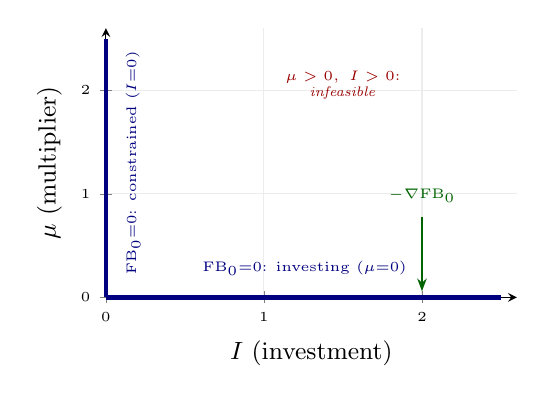
\begin{tikzpicture}
\begin{axis}[
    width=6.8cm, height=5.0cm,
    xlabel={$I$ (investment)}, ylabel={$\mu$ (multiplier)},
    label style={font=\small},
    tick label style={font=\tiny},
    xmin=0, xmax=2.6, ymin=0, ymax=2.6,
    xtick={0,1,2}, ytick={0,1,2},
    grid=major, grid style={gray!15},
    axis lines=left, clip=false,
    every axis plot/.append style={ultra thick, no markers},
]
    % FB_0 = 0 on the two positive half-axes
    \addplot[uzhblue, domain=0:2.5, samples=2] {0};
    \addplot[uzhblue, samples=2] coordinates {(0,0) (0,2.5)};
    % Open first quadrant = infeasible (violates complementarity)
    \node[font=\tiny, text=harvardcrimson, align=center] at (axis cs:1.5,2.05)
        {$\mu>0,\ I>0$:\\ \emph{infeasible}};
    % FB_0=0 labels on the half-axes
    \node[font=\tiny, text=uzhblue, anchor=west] at (axis cs:0.55,0.28)
        {$\mathrm{FB}_0{=}0$: investing ($\mu{=}0$)};
    \node[font=\tiny, text=uzhblue, rotate=90, anchor=south] at (axis cs:0.28,1.3)
        {$\mathrm{FB}_0{=}0$: constrained ($I{=}0$)};
    % loss-descent direction: in the interior FB_0>0, so -grad FB_0 points back to an axis
    \draw[-{Stealth[length=1.6mm]}, thick, darkgreen] (axis cs:2.0,0.78) -- (axis cs:2.0,0.06);
    \node[font=\tiny, darkgreen, anchor=south] at (axis cs:2.0,0.82) {$-\nabla\mathrm{FB}_0$};
\end{axis}
\end{tikzpicture}\\[2pt]
{\scriptsize $\mathrm{FB}_0{=}0$ exactly on the two blue half-axes (one of $\mu,I$ is zero, the other $\geq 0$). The open quadrant is infeasible; $-\nabla\mathrm{FB}_0$ (green) pushes a prediction there back to the nearest axis.}
\end{center}
\end{columns}
\end{frame}

% --- Slide 16: FOC: Consumption Sharing ---
\begin{frame}{FOC: Consumption Sharing}
\textbf{First-order condition} w.r.t.\ $c^j$:
\[
\tau^j \cdot (c^j)^{-1/\gamma_j} = \lambda
\]
where $\lambda$ is the \emphc{shadow price} of the aggregate resource constraint.

\vspace{0.5em}
\textbf{Solving for consumption:}
\[
\boxed{c^j = \left(\frac{\lambda}{\tau^j}\right)^{-\gamma_j}}
\]

\vspace{0.5em}
\begin{itemize}
    \item $\lambda$ is the \emphc{single} policy variable governing consumption allocation
    \item Higher $\lambda$ $\Rightarrow$ resources are scarcer $\Rightarrow$ lower consumption
    \item Countries with higher $\gamma_j$ (lower risk aversion) respond more to $\lambda$
\end{itemize}
\end{frame}

% --- Slide 15: FOC: Euler Equation ---
\begin{frame}{FOC: Euler Equation}
\textbf{First-order condition} w.r.t.\ $k^{j\prime}$:
\[
\lambda\,(1 + \Gamma_{k'}) = \beta\,\E{\lambda' \cdot \text{MPK}^{j\prime} - (1-\delta)\,\mu^{j\prime}} + \mu^j
\]

where:
\begin{itemize}
    \item $\Gamma_{k'} = \kappa\!\left(\frac{k'}{k} - 1\right)$ is the marginal adjustment cost
    \item $\text{MPK}^j = 1 - \delta + \zeta A_{\text{tfp}} \exp(z^j)\,(k^j)^{\zeta-1} - \frac{\partial \Gamma}{\partial k}$
    \item $\mu^j$ is the \emphc{irreversibility multiplier}
    \item The term $(1-\delta)\,\mu^{j\prime}$ captures the \emphc{shadow value} if the constraint binds tomorrow
\end{itemize}
\end{frame}

% --- Slide 16: Euler in Relative Error ---
\begin{frame}{Euler Equation: Relative Error Form}
Rearranging the Euler equation into \emphc{relative error} form:

\[
\boxed{
\frac{\beta\,\E{\lambda' \cdot \text{MPK}^{j\prime} - (1-\delta)\,\mu^{j\prime}} + \mu^j}{\lambda\,(1 + \Gamma_{k'})} - 1 = 0
}
\]

\vspace{0.5em}
\textbf{Why relative error?}
\begin{itemize}
    \item All $N$ Euler equations are \emphc{scale-free}
    \item Residuals can be interpreted as \emphc{percentage errors} in the optimality condition
    \item A residual of $10^{-3}$ means the agent is off by 0.1\%
\end{itemize}
\end{frame}

% --- Slide 17: Aggregate Resource Constraint ---
\begin{frame}{Aggregate Resource Constraint}
All output must be allocated to consumption, investment, and adjustment costs:

\[
\boxed{
\sum_{j=1}^{N} \Bigl[\underbrace{Y^j + (1-\delta)\,k^j}_{\text{resources}} - \underbrace{k^{j\prime}}_{\text{investment}} - \underbrace{\Gamma^j}_{\text{adj.\ cost}} - \underbrace{c^j}_{\text{consumption}}\Bigr] = 0
}
\]

\vspace{0.5em}
\begin{itemize}
    \item This is a \emphc{single} equation (not $N$ separate ones)
    \item Under complete markets, goods flow freely between countries
    \item Consumption $c^j$ is determined by $\lambda$ and the Pareto weights
\end{itemize}
\end{frame}

% --- Slide 18: Complementarity Conditions ---
\begin{frame}{Complementarity Conditions}
For each country $j$, the Fischer--Burmeister condition enforces irreversibility:

\[
\text{FB}_{\varepsilon}(\mu^j, I^j)
= \mu^j + I^j - \sqrt{(\mu^j)^2 + (I^j)^2 + \varepsilon^2} = 0
\]

where $I^j = k^{j\prime} - (1-\delta)\,k^j$.

\vspace{0.5em}
\textbf{Total system:}
\begin{center}
\begin{tabular}{lcc}
\toprule
\textbf{Equation} & \textbf{Count} & \textbf{Unknown} \\
\midrule
Euler equations & $N$ & $k^{1\prime}, \ldots, k^{N\prime}$ \\
Aggregate resource constraint & $1$ & $\lambda$ \\
Fischer--Burmeister & $N$ & $\mu^1, \ldots, \mu^N$ \\
\midrule
\textbf{Total} & $\bm{2N+1}$ & $\bm{2N+1}$ \\
\bottomrule
\end{tabular}
\end{center}
\end{frame}

% --- Slide 19: Summary: Equilibrium System ---
\begin{frame}{Summary: Equilibrium System}
\textbf{Well-posed system:} $2N+1$ equations in $2N+1$ unknowns.

\vspace{0.5em}
\begin{center}
\begin{tabular}{rrrr}
\toprule
$N$ & \textbf{States} & \textbf{Policies} & \textbf{Equations} \\
\midrule
2 & 4 & 5 & 5 \\
4 & 8 & 9 & 9 \\
10 & 20 & 21 & 21 \\
50 & 100 & 101 & 101 \\
100 & 200 & 201 & 201 \\
\bottomrule
\end{tabular}
\end{center}

\vspace{0.3em}
\begin{itemize}
    \item Dimensions grow \emphc{linearly} in $N$, no combinatorial explosion
    \item Traditional grid methods: $\mathcal{O}(n^{2N})$ grid points
    \item DEQNs: a single neural network, trained via SGD
\end{itemize}
\end{frame}

% --- Finger Exercise: IRBC ---
\begin{frame}{\exercisepause{} Finger Exercise: IRBC Euler Equations}
\begin{exampleblock}{Exercise}
Consider the 2-country IRBC model. Suppose we \emphc{double} the capital depreciation rate $\delta$ from the baseline $0.01$ to $0.02$.
\begin{enumerate}
    \item Without running any code: will the steady-state capital stock in each country \emph{increase} or \emph{decrease}? Why?
    \item Will the optimal savings rate (investment / output) increase or decrease?
    \item Open notebook \texttt{05\_01\_IRBC\_DEQN\_smooth.ipynb}, change $\delta$, and verify your prediction.
\end{enumerate}
\end{exampleblock}
\end{frame}

\begin{frame}{Solution: IRBC Euler Equations}
\begin{block}{Answer}
\begin{enumerate}
    \item Steady-state capital \emphc{decreases} \emph{if} $A_\mathrm{tfp}$ is held fixed at its $\delta = 0.01$ value: the Euler equation implies $r = 1/\beta - 1 + \delta$, so higher $\delta$ requires a higher marginal product of capital and (with diminishing returns) a lower $k^*$.  \textbf{Caveat:} the script's calibration normalizes $A_\mathrm{tfp} = (1/\beta - 1 + \delta)/\zeta$ so that $k_\mathrm{ss} = 1$ at the baseline; if you re-derive $A_\mathrm{tfp}$ at the new $\delta$, the normalized $k_\mathrm{ss}$ stays at $1$ and the change shows up in $A_\mathrm{tfp}$ itself and in the consumption--investment split.  The exercise asks for the \emph{$A_\mathrm{tfp}$-fixed} convention.
    \item The savings rate \emphc{increases}. More capital depreciates each period, so a larger fraction of output must be reinvested just to maintain the (lower) capital stock.
    \item In the notebook: changing $\delta$ from $0.01$ to $0.02$ should show the policy function shifting down (lower capital) and the investment share rising.
\end{enumerate}
\end{block}
\end{frame}

% ============================================================================
% PART II: DEQN FORMULATION
% ============================================================================

% --- Slide 20: Section Divider ---
\begin{frame}{}
\vfill
\begin{center}
{\Huge \textcolor{uzhblue}{\textbf{Part II}}}\\[12pt]
{\LARGE DEQN Formulation for the IRBC}
\end{center}
\vfill
\end{frame}

% --- Slide 21: State & Policy Variables ---
\begin{frame}{State \& Policy Variables}
\begin{center}
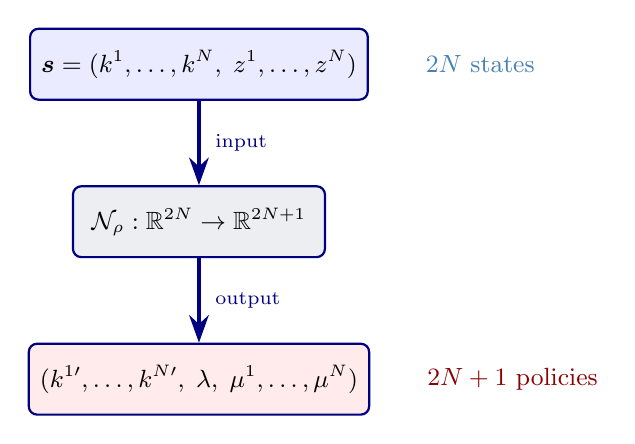
\begin{tikzpicture}[
    mlstep/.style={rectangle, draw=uzhblue, thick, fill=uzhgreylight,
        minimum width=3.2cm, minimum height=0.9cm, font=\small,
        rounded corners=3pt, inner sep=4pt},
    arr/.style={-{Stealth[length=3.5mm, width=2.5mm]}, very thick, uzhblue}
]
    \node[mlstep, fill=blue!8] (state) at (0, 0)
        {$\bm{s} = (k^1, \ldots, k^N,\; z^1, \ldots, z^N)$};
    \node[mlstep] (nn) at (0, -2.0)
        {$\mathcal{N}_\rho : \R^{2N} \to \R^{2N+1}$};
    \node[mlstep, fill=red!8] (policy) at (0, -4.0)
        {$(k^{1\prime}, \ldots, k^{N\prime},\; \lambda,\; \mu^1, \ldots, \mu^N)$};

    \draw[arr] (state) -- node[right, font=\scriptsize, uzhblue, xshift=2pt] {input} (nn);
    \draw[arr] (nn) -- node[right, font=\scriptsize, uzhblue, xshift=2pt] {output} (policy);

    \node[right=0.6cm, font=\small, softblue] at (state.east) {$2N$ states};
    \node[right=0.6cm, font=\small, darkred] at (policy.east) {$2N+1$ policies};
\end{tikzpicture}
\end{center}

\vspace{0.1em}
{\footnotesize\begin{itemize}\itemsep1pt
    \item The neural network maps the \emphc{full state} to \emphc{all policy variables simultaneously}
    \item For $N=2$: input dimension 4, output dimension 5
    \item Outputs must satisfy economic constraints: a \emphc{linear} output layer is mapped through custom per-policy transforms
\end{itemize}}
\end{frame}

% --- Slide 22: NN Architecture ---
\begin{frame}{Neural Network Architecture}
\begin{center}
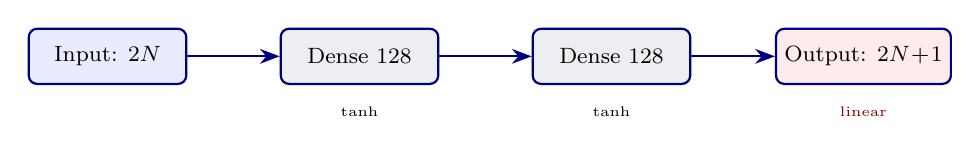
\begin{tikzpicture}[
    layer/.style={rectangle, draw=uzhblue, thick, fill=uzhgreylight,
        minimum width=2.0cm, minimum height=0.7cm, font=\footnotesize,
        rounded corners=3pt, inner sep=3pt},
    arr/.style={-{Stealth[length=2.5mm]}, thick, uzhblue}
]
    \node[layer, fill=blue!8] (in) at (0,0) {Input: $2N$};
    \node[layer] (h1) at (3.2,0) {Dense 128};
    \node[layer] (h2) at (6.4,0) {Dense 128};
    \node[layer, fill=red!8] (out) at (9.6,0) {Output: $2N\!+\!1$};

    \draw[arr] (in) -- (h1) node[midway, above, font=\tiny] {};
    \draw[arr] (h1) -- (h2) node[midway, above, font=\tiny] {};
    \draw[arr] (h2) -- (out) node[midway, above, font=\tiny] {};

    \node[below=0.15cm, font=\tiny] at (h1.south) {tanh};
    \node[below=0.15cm, font=\tiny] at (h2.south) {tanh};
    \node[below=0.15cm, font=\tiny, darkred] at (out.south) {linear};
\end{tikzpicture}
\end{center}

\vspace{0.5em}
\begin{itemize}
    \item \textbf{Hidden layers:} 2 layers $\times$ 128 units with \emphc{tanh} activation
    \item \textbf{Output layer:} \emphc{linear} (zero-initialized); raw outputs pass through custom transforms
    \item Transforms enforce the constraints: $k^{j\prime} > 0$ via $\exp\!\cdot\!\tanh$, $\lambda > 0$ via $\exp\!\cdot\!\tanh$, $\mu^j \geq 0$ via softplus (the smooth model omits $\mu^j$)
    \item Total parameters: $(2N \cdot 128 + 128) + (128 \cdot 128 + 128) + (128 \cdot (2N+1) + 2N+1)$
\end{itemize}
\end{frame}

% --- Slide 23: Enforcing positive outputs ---
\begin{frame}{Enforcing Positive, Feasible Outputs}
\begin{center}
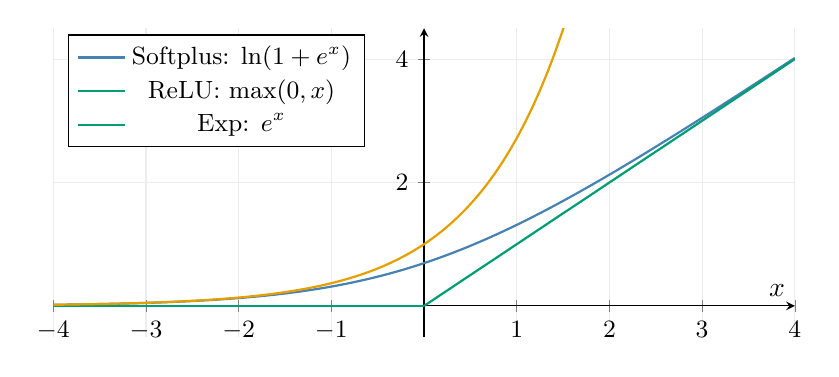
\begin{tikzpicture}
\begin{axis}[
    width=11cm, height=5.5cm,
    xlabel={$x$},
    xlabel style={font=\small},
    tick label style={font=\small},
    xmin=-4, xmax=4, ymin=-0.5, ymax=4.5,
    grid=major, grid style={gray!15},
    legend style={font=\small, at={(0.02,0.98)}, anchor=north west},
    axis lines=middle,
]
    \addplot[thick, softblue, domain=-4:4, samples=100]
        {ln(1+exp(x))};
    \addlegendentry{Softplus: $\ln(1+e^x)$}
    \addplot[thick, softgreen, domain=-4:0, samples=2]{0};
    \addplot[thick, softgreen, domain=0:4, samples=2]{x};
    \addlegendentry{ReLU: $\max(0,x)$}
    \addplot[thick, softorange, domain=-4:4, samples=100]
        {exp(x)};
    \addlegendentry{Exp: $e^x$}
\end{axis}
\end{tikzpicture}
\end{center}

\vspace{0.2em}
{\small
The notebooks keep a \emphc{linear} output and apply bounded transforms: $k^{j\prime}=k^j\exp\{\bar g\tanh r\}$ and $\lambda=\lambda_{\text{ref}}\exp\{s\tanh r\}$, the $\tanh$ caps the exponent, so no overflow (unlike a raw $e^x$), while the inequality multipliers $\mu^j$ use \textbf{softplus}.
}
\end{frame}

% --- Slide 24: DEQN Loss for IRBC ---
\begin{frame}{DEQN Loss Function for the IRBC}
\footnotesize
The loss is the \emphc{sum of squared residuals} across all equilibrium conditions; $\ell_\rho = 0$ iff every condition holds exactly.

\vspace{0.15em}
\textbf{Smooth benchmark} (notebook 04a):
\[
\boxed{
\ell^{\mathrm{smooth}}_\rho = \frac{1}{B}\sum_{i=1}^{B} \left[\sum_{j=1}^{N} \bigl(\text{Euler}_j^{(i)}\bigr)^2 + \bigl(\text{ARC}^{(i)}\bigr)^2\right]
}
\]

\vspace{0.1em}
\textbf{Irreversibility extension} (notebook 04b): add the Fischer--Burmeister block,
\[
\ell^{\mathrm{irrev}}_\rho = \ell^{\mathrm{smooth}}_\rho + \frac{1}{B}\sum_{i=1}^{B}\sum_{j=1}^{N}\bigl(\text{FB}_j^{(i)}\bigr)^2.
\]

\vspace{0.1em}
with $B$ the batch size:
\begin{itemize}\itemsep0pt
    \item $\text{Euler}_j = \dfrac{\beta\,\E{\lambda' \text{MPK}' - (1-\delta)\mu'} + \mu}{\lambda(1+\Gamma_{k'})} - 1$ \quad (smooth: $\mu \equiv 0$)
    \item $\text{ARC} = \sum_j [Y^j + (1-\delta)k^j - k^{j\prime} - \Gamma^j - c^j]$
    \item $\text{FB}_j = \mu^j + I^j - \sqrt{(\mu^j)^2 + (I^j)^2 + \varepsilon^2}$ \quad (\emph{04b only})
\end{itemize}
\end{frame}

% --- Slide 25: Gauss-Hermite Quadrature ---
\begin{frame}{Gauss--Hermite Quadrature}
\footnotesize
The Euler equation requires computing $\E{\cdot}$ over $N+1$ normal shocks.

\textbf{Gauss--Hermite quadrature} in 1D:
\[
\E{f(\varepsilon)} = \int f(\varepsilon)\, \phi(\varepsilon)\,d\varepsilon \approx \sum_{q=1}^{Q} w_q \, f(\varepsilon_q)
\]

\textbf{Tensor product} for $N+1$ dimensions:
\[
\E{f(\varepsilon^1, \ldots, \varepsilon^N, \varepsilon^{\text{agg}})} \approx \sum_{q_1=1}^{Q}\cdots\sum_{q_{N+1}=1}^{Q} \left(\prod_{d} w_{q_d}\right) f(\varepsilon_{q_1}, \ldots, \varepsilon_{q_{N+1}})
\]

\begin{center}
\begin{tabular}{rrrr}
\toprule
$N$ & \textbf{Shocks} & $Q$ & \textbf{Quad.\ nodes} \\
\midrule
2 & 3 & 3 & 27 \\
4 & 5 & 3 & 243 \\
10 & 11 & 3 & $\sim 177$K \\
\bottomrule
\end{tabular}
\end{center}

\vspace{0.2em}
{\footnotesize \textbf{What the companion notebooks do.} Both 04a and 04b use the \emphc{Stroud-3 monomial rule} ($2(N+1)$ nodes; $6$ for $N=2$), not the tensor-product Gauss--Hermite above; the latter is shown for contrast and is practical only at very low $N$.}
\end{frame}

% --- Slide 26: Computing Euler Expectation ---
\begin{frame}{Computing the Euler Expectation}
\textbf{Step-by-step} for each quadrature node $q$:

\vspace{0.3em}
\begin{enumerate}
    \item \textbf{Current state} $\bm{s}_t = (k^1, \ldots, k^N, z^1, \ldots, z^N)$
    \item \textbf{Current policy} $\mathcal{N}_\rho(\bm{s}_t) \to (k^{1\prime}, \ldots, k^{N\prime}, \lambda)$ \quad{\small(smooth, $N+1$ outputs; the irreversible extension appends $\mu^1, \ldots, \mu^N$)}
    \item \textbf{Next-period state} at node $q$:
    \[
    k^{j\prime}_q = k^{j\prime}, \qquad z^{j\prime}_q = \rho_z z^j + \sigma_e(\varepsilon^j_q + \varepsilon^{\text{agg}}_q)
    \]
    \item \textbf{Next-period policy:} evaluate $\mathcal{N}_\rho(\bm{s}_{t+1,q})$
    \item \textbf{Accumulate:} $\text{E-term} = \sum_q w_q \bigl[\lambda'_q \cdot \text{MPK}^j_q - (1-\delta)\mu^{j\prime}_q\bigr]$
\end{enumerate}

\vspace{0.3em}
{\small Each quadrature node requires a \emphc{forward pass} through the network, but all nodes in a batch can be evaluated in parallel.}
\end{frame}

% --- Slide 27: State Transition ---
\begin{frame}{State Transition}
\begin{center}
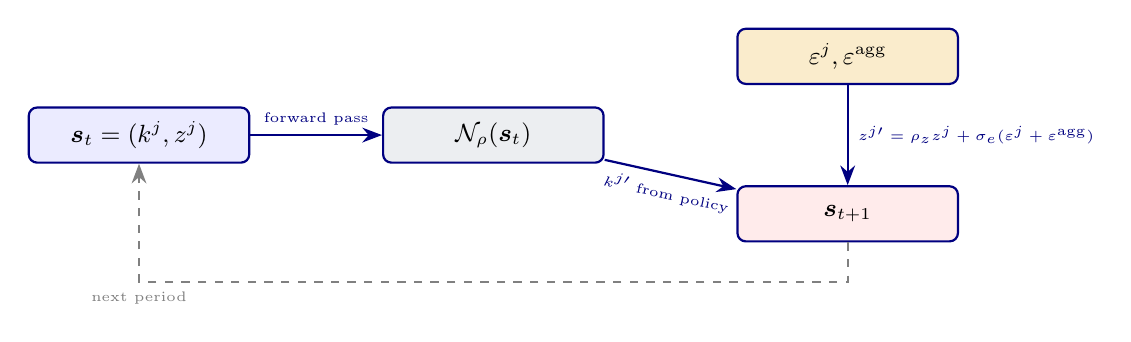
\begin{tikzpicture}[
    mlstep/.style={rectangle, draw=uzhblue, thick, fill=uzhgreylight,
        minimum width=2.8cm, minimum height=0.7cm, font=\small,
        rounded corners=3pt, inner sep=3pt},
    arr/.style={-{Stealth[length=2.5mm]}, thick, uzhblue}
]
    \node[mlstep, fill=blue!8] (st) at (0,0) {$\bm{s}_t = (k^j, z^j)$};
    \node[mlstep] (nn) at (4.5,0) {$\mathcal{N}_\rho(\bm{s}_t)$};
    \node[mlstep, fill=softorange!20] (shock) at (9,1) {$\varepsilon^j, \varepsilon^{\text{agg}}$};
    \node[mlstep, fill=red!8] (st1) at (9,-1) {$\bm{s}_{t+1}$};

    \draw[arr] (st) -- (nn) node[midway, above, font=\tiny] {forward pass};
    \draw[arr] (nn) -- (st1) node[midway, below, font=\tiny, sloped] {$k^{j\prime}$ from policy};
    \draw[arr] (shock) -- (st1) node[midway, right, font=\tiny] {$z^{j\prime} = \rho_z z^j + \sigma_e(\varepsilon^j + \varepsilon^{\text{agg}})$};

    \draw[arr, dashed, gray] (st1.south) -- ++(0,-0.5) -| (st.south)
        node[midway, below, font=\tiny, text=gray] {next period};
\end{tikzpicture}
\end{center}

\vspace{0.5em}
\begin{itemize}
    \item \textbf{Capital:} $k^{j\prime}$ is a policy output (endogenous)
    \item \textbf{TFP:} $z^{j\prime}$ evolves exogenously via AR(1) + shocks
    \item For simulation: draw $\varepsilon \sim \mathcal{N}(0,1)$
    \item For expectations: use quadrature nodes $\varepsilon_q$
\end{itemize}
\end{frame}

% --- Slide 28: Training Algorithm ---
\begin{frame}{Training Algorithm}
\begin{block}{Algorithm 1: DEQN Training for IRBC (persistent simulation)}
\begin{algorithmic}
\footnotesize
\STATE \textbf{Input:} Network $\mathcal{N}_\rho$, learning rate $\eta$, segments $S$, monomial nodes/weights
\STATE Initialize $M$ trajectory heads $\bm{X}^{(1)}, \ldots, \bm{X}^{(M)}$ from a feasible starting cloud
\FOR{segment $s = 1, \ldots, S$}
    \STATE Simulate: for $t = 1, \ldots, T$, sample shocks and step each head one period under $\mathcal{N}_\rho$
    \STATE Flatten the $M\!\cdot\!T$ recorded states into a training batch
    \FOR{pass $p = 1, \ldots, P$ \textbf{ over mini-batches of the segment}}
        \STATE Compute loss $\ell_\rho$ on the segment (smooth: Euler + ARC; irreversible: also FB)
        \STATE Update: $\rho \leftarrow \rho - \eta\,\nabla_\rho \ell_\rho$ (Adam)
    \ENDFOR
    \STATE Continue: $\bm{X}^{(m)} \leftarrow$ terminal state of trajectory $m$ (\emph{no reset to steady state})
    \STATE \textbf{Monitor:} policy drift on \texttt{X\_anchor}; flag stable when below tolerance
\ENDFOR
\STATE \textbf{Diagnostic:} zero-shock SSS check from dispersed feasible starts
\STATE \textbf{Output:} Trained $\mathcal{N}_{\rho^\star}$
\end{algorithmic}
\end{block}
\end{frame}

% --- Slide 29: Scalability in N ---
\begin{frame}{Scalability in $N$}
\begin{center}
\begin{tabular}{rrrrl}
\toprule
$N$ & \textbf{States} & \textbf{Policies} & \textbf{NN params} & \textbf{Grid pts ($n\!=\!10$)} \\
\midrule
2 & 4 & 5 & $\sim$4.8K & $10^4$ \\
4 & 8 & 9 & $\sim$5.3K & $10^8$ \\
10 & 20 & 21 & $\sim$6.9K & $10^{20}$ \\
50 & 100 & 101 & $\sim$17K & $10^{100}$ \\
100 & 200 & 201 & $\sim$30K & $10^{200}$ \\
\bottomrule
\end{tabular}
\end{center}

\vspace{0.5em}
\begin{itemize}
    \item NN parameters grow \emphc{linearly} in $N$ (only input/output layers scale)
    \item Grid methods grow \emphc{exponentially}: $10^{2N}$ points
    \item DEQN training cost per step: $\mathcal{O}(|\rho| \cdot B \cdot Q^{N+1})$
    \item For large $N$: replace tensor-product GH with monomial rules or QMC
    \item Theoretical underpinning: \emphc{deep ReLU networks} beat the curse of dimensionality for sparse-grid-representable functions (Montanelli \& Du 2019)
\end{itemize}
\end{frame}

% --- Slide 30: From Brock-Mirman to IRBC ---
% --- Padova cut: frame "From Brock--Mirman to IRBC" (21 lines) commented out ---
% \begin{frame}{From Brock--Mirman to IRBC}
% \begin{center}
% \begin{tabular}{lll}
% \toprule
% & \textbf{Brock--Mirman} & \textbf{IRBC} \\
% \midrule
% Countries & 1 & $N$ \\
% States & $(K, z)$ & $(k^1, \ldots, k^N, z^1, \ldots, z^N)$ \\
% Policies & $C$ (or $s$) & $(k^{1\prime}, \ldots, k^{N\prime}, \lambda, \mu^1, \ldots, \mu^N)$ \\
% Equations & 1 Euler & $N$ Euler $+$ 1 ARC $+$ $N$ FB \\
% Constraints & none & irreversibility, adj.\ costs \\
% Shocks & 1 & $N+1$ \\
% Output act. & sigmoid & linear $+$ transforms \\
% Analytical sol. & yes ($\delta=1$) & no \\
% \bottomrule
% \end{tabular}
% \end{center}
% 
% \vspace{0.3em}
% {\small The IRBC is a natural \emphc{scaling test} for the DEQN methodology.}
% \end{frame}

% --- Slide 31: Recap ---
\begin{frame}{Recap: Three Building Blocks}
\begin{columns}[T]
\column{0.32\textwidth}
\begin{block}{Model}
\centering
\small
$N$-country IRBC with irreversible investment, adjustment costs, complete markets. $2N+1$ equilibrium equations.
\end{block}

\column{0.32\textwidth}
\begin{block}{Network}
\centering
\small
$\mathcal{N}_\rho: \R^{2N} \to \R^{2N+1}$ with tanh hidden layers, linear output mapped through bounded transforms. All policies in one forward pass.
\end{block}

\column{0.32\textwidth}
\begin{block}{Training}
\centering
\small
Persistent simulation: one continuing trajectory ensemble, Adam on the sum of squared residuals.
\end{block}
\end{columns}

\vspace{0.5em}
{\small \textbf{Relative to Brock--Mirman:} one country $\to N$; state $(K,z)\to(k^{1:N},z^{1:N})$;
one Euler equation $\to N$ Euler $+$ 1 ARC $+$ $N$ Fischer--Burmeister; a closed form (at $\delta=1$)
$\to$ none. The IRBC is the natural \emphc{scaling test} for the method.}

\vspace{0.4em}
\begin{center}
$\Rightarrow$ \textbf{Next:} implementation in TensorFlow/Keras and results.
\end{center}
\end{frame}

% ============================================================================
% PART III: IMPLEMENTATION & RESULTS
% ============================================================================

% --- Slide 32: Section Divider ---
\begin{frame}{}
\vfill
\begin{center}
{\Huge \textcolor{uzhblue}{\textbf{Part III}}}\\[12pt]
{\LARGE Implementation \& Results}
\end{center}
\vfill
\end{frame}

% --- Slide 33: Notebook Overview ---
\begin{frame}{Notebook Overview}
\scriptsize
\textbf{Three notebooks accompany this lecture} (two in the L04 \texttt{code/} folder, one in the L05 folder; self-contained, all equations inline):

\vspace{0.2em}
\begin{enumerate}\itemsep1pt
    \item \texttt{05\_01\_IRBC\_DEQN\_smooth.ipynb}, \emph{smooth benchmark, in-class walk-through (this lecture's \texttt{code/})}
    \begin{itemize}\itemsep0pt
        \item Parameters \& steady state, monomial quadrature; Keras network, production/consumption/adjustment-cost equations
        \item Cost function (Euler + ARC), persistent-simulation training loop
        \item Time-invariance check and zero-shock stochastic steady state
    \end{itemize}

    \item \texttt{05\_02\_IRBC\_DEQN\_irreversible.ipynb}, \emph{irreversible-investment extension (this lecture's \texttt{code/})}
    \begin{itemize}\itemsep0pt
        \item KKT multipliers $\mu^j$ and feasibility-by-construction policy; Fischer--Burmeister complementarity loss
        \item Same training loop and diagnostics as the smooth benchmark
    \end{itemize}

    \item \texttt{05\_03\_IRBC\_Exercise.ipynb}, \emph{hands-on exercise}
    \begin{itemize}\itemsep0pt
        \item Task 1: comparative statics on the deterministic steady state
        \item Task 2: inverse-loss weighting for multi-component losses (ReLoBRaLo, from Session 3)
    \end{itemize}
\end{enumerate}
\end{frame}

% --- Slide 34: Parameters ---
\begin{frame}{Parameters}
\begin{center}
\begin{tabular}{llrl}
\toprule
\textbf{Symbol} & \textbf{Name} & \textbf{Value} & \textbf{Description} \\
\midrule
$\beta$ & Discount factor & 0.99 & Quarterly calibration \\
$\zeta$ & Capital share & 0.36 & Cobb--Douglas \\
$\delta$ & Depreciation & 0.01 & Low depreciation \\
$\rho_z$ & TFP persistence & 0.95 & Highly persistent \\
$\sigma_e$ & Shock std.\ dev. & 0.01 & Small shocks \\
$\kappa$ & Adjustment cost & 0.50 & Moderate costs \\
$\gamma_{\min}$ & Min IES & 0.25 & High risk aversion \\
$\gamma_{\max}$ & Max IES & 1.00 & Log utility \\
$k_{ss}$ & Steady-state capital & 1.00 & Normalization \\
\bottomrule
\end{tabular}
\end{center}

\vspace{0.3em}
{\small Pareto weights: $\tau^j = (A_{\text{tfp}} - \delta)^{1/\gamma_j} = c_{ss}^{1/\gamma_j}$.  At the symmetric steady state $c_{ss} = A_{\text{tfp}} - \delta$ for every country, so $\lambda_{ss} = \tau^j (c_{ss})^{-1/\gamma_j} = 1$ shared across all $j$ regardless of heterogeneous $\gamma_j$.}
\end{frame}

% --- Slide 35: Steady State ---
\begin{frame}{Steady State}
At steady state ($z^j = 0$, $k^j = k_{ss} = 1$, $\mu^j = 0$):

\vspace{0.3em}
\begin{align*}
A_{\text{tfp}} &= \frac{1 - \beta(1-\delta)}{\zeta\beta} = \frac{1 - 0.99 \cdot 0.99}{0.36 \cdot 0.99} \approx 0.0559 \\[4pt]
Y_{ss} &= A_{\text{tfp}} \cdot k_{ss}^\zeta = A_{\text{tfp}} \approx 0.0559 \\[4pt]
I_{ss} &= \delta \cdot k_{ss} = 0.01 \\[4pt]
c_{ss} &= Y_{ss} - I_{ss} \approx 0.0459
\end{align*}

\vspace{0.3em}
\textbf{Verification:} the ARC should be satisfied: $\sum_j [Y_{ss} - I_{ss} - c_{ss}] = 0$ \checkmark

\vspace{0.3em}
{\small The Euler equation at steady state gives the MPK $= 1/\beta$, which pins down $A_{\text{tfp}}$.}
\end{frame}

% --- Slide 36: Network Definition (Code) ---
% --- Padova cut: frame "Network Definition (Keras)" (26 lines) commented out ---
% \begin{frame}[fragile]{Network Definition (Keras)}
% \begin{center}
% \begin{minipage}{0.85\textwidth}
% \begin{lstlisting}
% N_COUNTRIES = 2
% n_states = 2 * N_COUNTRIES      # = 4
% n_policies = 2 * N_COUNTRIES + 1 # = 5
% 
% nn = keras.Sequential([
%     keras.layers.Dense(128, activation='tanh',
%                        input_shape=(n_states,)),
%     keras.layers.Dense(128, activation='tanh'),
%     keras.layers.Dense(n_policies, activation=None,
%                        kernel_initializer='zeros')
% ])
% \end{lstlisting}
% \end{minipage}
% \end{center}
% 
% \vspace{0.3em}
% \begin{itemize}
%     \item \texttt{tanh} hidden activations; output layer is linear (zero-initialized)
%     \item Raw outputs pass through custom transforms (\texttt{exp$\cdot$tanh}, \texttt{sigmoid}, \texttt{softplus}) to enforce the constraints
%     \item Output: $[k^{1\prime}, k^{2\prime}, \lambda, \mu^1, \mu^2]$
% \end{itemize}
% \end{frame}

% --- Slide 37: Production & Consumption (Code) ---
% --- Padova cut: frame "Production \& Consumption" (26 lines) commented out ---
% \begin{frame}[fragile]{Production \& Consumption}
% \begin{columns}[T]
% \column{0.48\textwidth}
% \textbf{Production:}
% \begin{lstlisting}[basicstyle=\footnotesize\ttfamily]
% def production(k, z):
%     return A_tfp * tf.exp(z) \
%            * k**zeta
% \end{lstlisting}
% 
% $Y^j = A_{\text{tfp}} \exp(z^j) (k^j)^\zeta$
% 
% \column{0.48\textwidth}
% \textbf{Consumption (from FOC):}
% \begin{lstlisting}[basicstyle=\footnotesize\ttfamily]
% def consumption(lamb, j):
%     tau = (A_tfp - delta)**(1./gammas[j])
%     return (lamb/tau)**(-gammas[j])
% \end{lstlisting}
% 
% $c^j = (\lambda / \tau^j)^{-\gamma_j}$
% \end{columns}
% 
% \vspace{0.5em}
% {\small All functions are vectorized over the batch dimension using TensorFlow operations.}
% \end{frame}

% --- Slide 38: Adjustment Costs (Code) ---
% --- Padova cut: frame "Adjustment Costs" (23 lines) commented out ---
% \begin{frame}[fragile]{Adjustment Costs}
% \begin{lstlisting}
% def adj_cost(k, kp):
%     j = kp / k - 1.0
%     return 0.5 * kappa * j**2 * k
% 
% def adj_cost_kp(k, kp):
%     return kappa * (kp / k - 1.0)
% 
% def adj_cost_k(k, kp):
%     j = kp / k - 1.0
%     return -0.5 * kappa * j * (j + 2.0)
% \end{lstlisting}
% 
% \vspace{0.3em}
% \textbf{Marginal product of capital:}
% \begin{lstlisting}
% def mpk(k, z, kp):
%     Fk = zeta * A_tfp * tf.exp(z) \
%          * k**(zeta - 1)
%     return 1 - delta + Fk - adj_cost_k(k, kp)
% \end{lstlisting}
% \end{frame}

% --- Slide 39: Fischer-Burmeister (Code) ---
\begin{frame}[fragile]{Fischer--Burmeister Function}
\begin{lstlisting}
def fischer_burmeister(mu, I, eps=1e-4):
    return mu + I - tf.sqrt(mu**2 + I**2 + eps**2)
\end{lstlisting}

\vspace{0.3em}
\textbf{Investment:}
\begin{lstlisting}
def investment(k, kp):
    return kp - (1.0 - delta) * k
\end{lstlisting}

\vspace{0.3em}
The FB function is:
\begin{itemize}
    \item \emphc{Differentiable} everywhere for $\varepsilon>0$ (unlike $\min(\mu, I)$)
    \item \emphc{Exact zero set} at $\varepsilon=0$: $\mu \geq 0$, $I \geq 0$, $\mu \cdot I = 0$
    \item The small $\varepsilon$ prevents division-by-zero at the origin
\end{itemize}
\end{frame}

% --- Slide 40: Cost Function Structure ---
\begin{frame}[fragile]{Cost Function Structure}
\begin{lstlisting}[basicstyle=\footnotesize\ttfamily]
@tf.function
def compute_cost(states, nn):
    policies = nn(states)
    # Extract k', lambda, mu per country
    # For each GH quadrature node:
    #   Compute next state, evaluate nn,
    #   accumulate Euler integrand
    # Euler residual (relative error)
    # ARC: sum resources - uses = 0
    # FB: complementarity per country
    loss = mean(euler**2 + arc**2 + fb**2)
    return loss
\end{lstlisting}

\vspace{0.3em}
\textbf{Key point:} the entire computation graph is inside \texttt{@tf.function} for \emphc{automatic differentiation} via \texttt{GradientTape}.
\end{frame}

% --- Slide 41: Persistent-Simulation Training ---
\begin{frame}{Persistent-Simulation Training}
\vspace{-2pt}
The companion notebooks train on \emphc{one continuing trajectory ensemble}, no Phase~1 / Phase~2 switch, no resets to steady state.

\vspace{0.15em}
\begin{itemize}
    \item Maintain $M = \texttt{N\_TRAJECTORIES}$ stochastic trajectory heads $\bm{X}^{(1)}, \ldots, \bm{X}^{(M)}$.
    \item Each \emphc{training segment}: simulate the heads forward for $T = \texttt{SIMULATION\_LENGTH}$ stochastic periods under the \emph{current} policy network; flatten into a training cloud of size $M\!\cdot\!T$; perform a fixed number of SGD passes.
    \item Continue from the segment's terminal states: $\bm{X}_{\mathrm{start}} \leftarrow \bm{X}_{\mathrm{end}}$. The trajectory ensemble \emphc{co-evolves} with the policy.
    \item A \texttt{SAMPLING\_MODE} switch (\texttt{simulation} vs \texttt{exogenous}) is available for ablations; the default \texttt{simulation} mode never sees a uniform burn-in.
\end{itemize}

\vspace{0.15em}
\textbf{Why this works without a separate burn-in.}
\begin{itemize}
    \item The policy parameterization is feasibility-bounded by construction:
    \begin{itemize}\itemsep1pt
        \item smooth (04a): $k^{j\prime} = k^j \exp\{\bar g \tanh r_j(\bm{s})\}$ keeps $k^{j\prime} > 0$;
        \item irreversible (04b): $k^{j\prime} = (1-\delta)k^j + I^j$ with $I^j \ge 0$ enforced via a sigmoid head.
    \end{itemize}
    \item Random initial weights cannot drive the simulation into infeasible states.
\end{itemize}
\end{frame}

% --- Slide 42: Diagnostics: Time-Invariance and Zero-Shock SSS ---
\begin{frame}{Diagnostics: Time-Invariance and Zero-Shock SSS}
\textbf{Time invariance.}  The architecture has no calendar-time input, so any fixed weight vector defines a stationary recursive policy.  The \emph{numerical} question is whether SGD has stopped moving the policy function.

\vspace{0.2em}
\begin{itemize}
    \item Evaluate the policy on a fixed anchor cloud \texttt{X\_anchor} after each monitoring interval.
    \item Report \texttt{policy\_drift\_rms} and \texttt{policy\_drift\_max}.
    \item When both fall below \texttt{TIME\_INVARIANCE\_TOL\_RMS} / \texttt{\_MAX}, the run is flagged \emphc{stable}.
\end{itemize}

\vspace{0.3em}
\textbf{Zero-shock stochastic steady state (SSS).}  Iterate the learned policy from \texttt{ZERO\_SHOCK\_N\_STARTS} dispersed feasible starts with $\varepsilon^j_t = \varepsilon^{\mathrm{agg}}_t = 0$.

\vspace{0.2em}
\begin{itemize}
    \item All paths should converge to a common point.
    \item In a sensible SSS: $I^j \approx \delta\,k^j$ (investment replaces depreciation) and, in 04b, the irreversibility multiplier $\mu^j \approx 0$.
\end{itemize}
\end{frame}

% --- Slide 43: Persistent-Simulation Training: What to Monitor ---
\begin{frame}{Persistent-Simulation Training: What to Monitor}
With a single training pipeline (no Phase~1/Phase~2 switch), \emph{four} signals carry the whole convergence story:

\vspace{0.3em}
\begin{enumerate}\itemsep3pt
    \item \textbf{Total loss} decays monotonically across training segments (the \emph{loss-vs-segment} panel in the notebooks).
    \item \textbf{Per-residual mean magnitudes}: \texttt{mean\_abs\_euler}, \texttt{mean\_abs\_arc}, and (in 04b) \texttt{mean\_abs\_fb}, all fall below the prescribed tolerance.
    \item \textbf{Policy drift on the anchor cloud} crosses from \emphc{moving} to \emphc{stable}: only then is the policy time-invariant in the recursive sense.
    \item \textbf{Zero-shock SSS} converges from dispersed feasible starts to a common point with $I^j \to \delta\,k^j$ and (in 04b) $\mu^j \to 0$.
\end{enumerate}

\vspace{0.4em}
{\footnotesize \emph{Historical note.}  An earlier four-approach comparison (uniform vs simulation-only vs two-phase vs ReLoBRaLo) on the same model is preserved in \texttt{figures/irbc\_4approach\_loss.pdf}; it is \emph{not} produced by the current notebooks, which run a single persistent-simulation pipeline.}
\end{frame}

% --- Slide 44: Convergence: Per-Equation ---
\begin{frame}{Convergence: Per-Equation Residuals}
\textbf{After training}: we evaluate residuals on a test cloud (smooth + irreversible):

\vspace{0.5em}
\begin{center}
\begin{tabular}{lcc}
\toprule
\textbf{Residual} & \textbf{Mean $|\cdot|$} & \textbf{Max $|\cdot|$} \\
\midrule
Euler (country 1) & $\sim 10^{-4}$ & $\sim 10^{-3}$ \\
Euler (country 2) & $\sim 10^{-4}$ & $\sim 10^{-3}$ \\
ARC & $\sim 10^{-4}$ & $\sim 10^{-3}$ \\
\midrule
\multicolumn{3}{l}{\textit{Irreversibility extension (notebook 04b only):}} \\
FB (country 1) & $\sim 10^{-5}$ & $\sim 10^{-4}$ \\
FB (country 2) & $\sim 10^{-5}$ & $\sim 10^{-4}$ \\
\bottomrule
\end{tabular}
\end{center}

\vspace{0.3em}
\begin{itemize}
    \item Euler residuals $< 10^{-3}$ $\Rightarrow$ policy is accurate to within 0.1\%
    \item FB residuals near zero $\Rightarrow$ complementarity is well satisfied (04b only)
    \item These are \emphc{relative errors}, interpretable as percentage deviations
\end{itemize}
\end{frame}

% --- Slide 45: Policy Functions ---
\begin{frame}{Policy Functions}
\textbf{After training,} we visualize the learned policies:

\vspace{0.3em}
\begin{columns}[T]
\column{0.48\textwidth}
\begin{itemize}
    \item \textbf{Capital policy} $k^{j\prime}$ vs.\ $k^j$:
    \begin{itemize}
        \item Near 45-degree line (close to replacement)
        \item Higher investment when TFP is high
    \end{itemize}
    \vspace{0.3em}
    \item \textbf{Shadow price} $\lambda$ vs.\ $z^j$:
    \begin{itemize}
        \item Decreasing in productivity (more output $\Rightarrow$ lower scarcity)
    \end{itemize}
\end{itemize}

\column{0.48\textwidth}
\begin{itemize}
    \item \textbf{Multiplier} $\mu^j$ vs.\ $k^j$:
    \begin{itemize}
        \item Near zero when $k$ is low (investment is positive)
        \item Positive when $k$ is high (irreversibility binds)
    \end{itemize}
    \vspace{0.3em}
    \item \textbf{Investment} $I^j$ vs.\ $k^j$:
    \begin{itemize}
        \item Positive most of the time
        \item Occasionally zero (constraint active)
    \end{itemize}
\end{itemize}
\end{columns}
\end{frame}

% --- Slide 46: Economic Diagnostics ---
\begin{frame}{Economic Diagnostics}
\footnotesize
\begin{columns}[T]
\column{0.48\textwidth}
\textbf{Consumption sharing:}
\begin{itemize}\itemsep1pt
    \item Under complete markets, $c^1$ and $c^2$ should be \emphc{positively correlated}
    \item Perfect risk sharing: $c^1/c^2$ is constant
    \item With heterogeneous $\gamma$: ratio varies with $\lambda$
\end{itemize}

\vspace{0.2em}
{\footnotesize Reconnects with the \emphc{consumption-correlation puzzle} from slide~7: complete markets predict $\rho(c^1,c^2)\!\approx\!1$, but in data $\rho(c^1,c^2)<\rho(y^1,y^2)$; closing the gap needs incomplete markets or frictions.}

\vspace{0.2em}
\textbf{Trade balance:}
\begin{itemize}\itemsep1pt
    \item $\text{TB}^j = Y^j - c^j - I^j - \Gamma^j$ ($>0$ when $j$ exports)
    \item Sums to zero across countries
\end{itemize}

\column{0.48\textwidth}
\textbf{Ergodic distribution:}
\begin{itemize}\itemsep1pt
    \item Scatter plot of $(k^1, k^2)$ over long simulation
    \item Should concentrate near $(k_{ss}, k_{ss})$
    \item Correlation structure reveals risk-sharing patterns
\end{itemize}

\vspace{0.5em}
\textbf{Complementarity check:}
\begin{itemize}\itemsep1pt
    \item Plot $\mu^j$ vs.\ $I^j$
    \item Should lie on the axes: $\mu = 0$ or $I = 0$
    \item Fraction of time constraint binds
\end{itemize}
\end{columns}
\end{frame}

% --- Slide 47: Validation ---
\begin{frame}{Validation: Euler LHS vs.\ RHS}
\textbf{Key diagnostic:} compare both sides of the Euler equation on a test set.

\vspace{0.5em}
\begin{columns}[T]
\column{0.48\textwidth}
\textbf{LHS:} $\lambda \cdot (1 + \Gamma_{k'})$

\vspace{0.3em}
\textbf{RHS:} $\beta\,\E{\lambda' \cdot \text{MPK}' - (1-\delta)\mu'} + \mu$

\vspace{0.5em}
\textbf{Targets:}
\begin{itemize}
    \item Points should lie on the \emphc{45-degree line}
    \item Mean relative error $< 10^{-3}$
    \item Max relative error $< 10^{-2}$
\end{itemize}

\column{0.48\textwidth}
\textbf{Also check:}
\begin{itemize}
    \item ARC residual $\approx 0$ across all states
    \item $\mu^j \approx 0$ whenever $I^j > 0$ (complementarity)
    \item $I^j \geq 0$ everywhere (irreversibility)
\end{itemize}

\vspace{0.5em}
{\small These diagnostics confirm the network has learned a valid \emphc{approximate equilibrium}.}
\end{columns}
\end{frame}

% --- Bridge frame ---
\begin{frame}{Bridge: from solving to estimating}
\footnotesize
\textbf{What we leave with today.}  An IRBC DEQN trained with a single persistent-simulation
pipeline and equal loss weights: the same recipe scales from $N=2$ to $N=10$ countries with no
architectural change.  NAS-tuned width and ReLoBRaLo-balanced loss components, from Session 3 this
afternoon, are the refinements to reach for when the equal-weight recipe stalls.

\vspace{0.4em}
\begin{columns}[T]
\column{0.48\textwidth}
\textbf{Day 1, in one line.}
\begin{itemize}
    \item The equilibrium residual \emph{is} the loss (Session 2).
    \item Architecture and loss weights are the two knobs that decide whether training works
          (Session 3).
    \item Cohorts and constraints do not change the principle (Session 4); neither does a
          $2N$-dimensional state (today).
\end{itemize}

\column{0.48\textwidth}
\textbf{Tomorrow.}
\begin{itemize}
    \item Solving is not the end: a trained solver is expensive to re-run. Deep surrogates and
          Gaussian processes \emph{amortize} it (Session 6).
    \item That makes structural estimation tractable (Session 7).
    \item Then the same residual idea in continuous time: PDEs, HJB, and the coupled HJB--KFE
          system (Sessions 8--9).
\end{itemize}
\end{columns}
\end{frame}

% --- Slide 49: Questions ---
\begin{frame}{}
\begin{columns}[c]
\column{0.45\textwidth}
\begin{center}
{\Huge \textcolor{uzhblue}{\textbf{Questions?}}}

\vspace{1.0cm}
{\large Simon Scheidegger}\\[4pt]
{\small HEC, University of Lausanne}\\[4pt]
\url{https://sischei.github.io}

\vspace{0.6cm}
{\small Materials:~~\url{https://github.com/sischei/deep_learning_padova_0926}}
\end{center}

\column{0.45\textwidth}
\begin{center}
\textbf{Next up:}\\[6pt]
{\large AutoDiff $\to$ Sequence Space $\to$\\[2pt]
OLG $\to$ Heterogeneous Agents (Young's method)}
\end{center}
\end{columns}
\end{frame}

\end{document}
